
%% Author: Egill B�i Einarsson
%% PTG, Parsing Table Generator
%% See copyleft below or in the generated document.

\documentclass[11pt,a4paper]{article}

\usepackage[american]{babel}
\usepackage[pdftex]{hyperref}
\usepackage{times}
\usepackage{float}
\usepackage[T1]{fontenc}
\usepackage[margin=1in]{geometry}
\usepackage{amsmath}
\usepackage{listings}
\usepackage{graphicx}
\usepackage{framed}
\usepackage{fancyvrb}
\usepackage{tikz}
\usetikzlibrary{arrows,automata}
\usetikzlibrary{shapes.multipart}
\usetikzlibrary{shapes.misc}

\newcommand{\plist}[1]{\hspace{10mm}
	\indent\parbox{14cm}{#1}
	\\ }

\begin{document}

\sloppy
\VerbatimFootnotes
\renewcommand{\arraystretch}{1.5}

%% This is currently unused and therefore empty.


\title{PTG User Manual}
\author{Egill B�i Einarsson}
\maketitle

\begin{abstract}
PTG is a command-line program that generates files containing parsing tables and state machines for a formal language defined by an input grammar. Generated tables are in either \LaTeX{} or HTML format which eases automated inserting of generated elements. Likewise the state machines can be inserted directly into the \LaTeX{} source files when the TIKZ format is used. Alternatively state machines can use Graphviz's digraph automaton format which is intended for use with Graphviz DOT.
\end{abstract}

\section*{Copyleft}
This program is free software: you can redistribute it and/or modify
it under the terms of the GNU General Public License as published by
the Free Software Foundation, either version 3 of the License, or
(at your option) any later version.


This program is distributed in the hope that it will be useful,
but WITHOUT ANY WARRANTY; without even the implied warranty of
MERCHANTABILITY or FITNESS FOR A PARTICULAR PURPOSE.  See the
GNU General Public License for more details.


You should have received a copy of the GNU General Public License
along with this program.  If not, see <\href{http://www.gnu.org/licenses/}{http://www.gnu.org/licenses/}>.
\newpage
\tableofcontents
\newpage
\section{Introduction}

PTG is run from a command-line terminal and generates parsing tables and state machines for context insensitive formal grammars. A grammar's FIRST, FOLLOW, LL(1), SLR(1), LALR(1) and LR(1) parsing tables can be generated in either \LaTeX{} or HTML format along with LR(0) and LR(1) state machines in Graphviz's digraph automaton format for use with DOT or TIKZ format for use directly in \LaTeX{}. The idea is when creating a document studying formal languages, that features some or all of these tables and machines, instead of writing the entites directly or copying a generated file into the master file, PTG generated files can be dynamically linked in the master file. The result is that if the formal languages change then only the PTG grammar file needs to be updated and then the tables and state machines can be represented by using PTG, Graphviz, etc.. This process can of course be automated with a make or batch file with the exception of updating the grammar file.

\section{Setup}

Setup is simple as long as a JRE (Java Runtime Environment) has been setup. Go to the \href{https://github.com/EgillEinarss/PTG}{PTG repository}\footnote{\verb| https://github.com/EgillEinarss/PTG|} on Github.com and download PTG.jar. Place this file in the current command line directory and run:

\begin{lstlisting}[frame=single]
java -jar PTG.jar ...
\end{lstlisting}

\noindent Along with any relevant arguments (detailed in the next section).

\subsection{Compiling the Source}

Required programs are \href{http://git-scm.com/}{git}\footnote{\verb| http://git-scm.com/|} and \href{http://www.gnu.org/software/make/}{make}\footnote{\verb| http://www.gnu.org/software/make/|}.
Use a command line. If needed, go to your projects directory and get the project with the command:

\begin{lstlisting}[frame=single]
git clone https://github.com/EgillEinarss/PTG.git
cd PTG
\end{lstlisting}

\noindent Alternatively go to the \href{https://github.com/EgillEinarss/PTG}{PTG repository} on \href{https://github.com/}{Github.com}\footnote{\verb| https://github.com/|} and download what you want or require.

Now the developement environment used to create PTG has been set up. To compile the source and create the jarfile used to run PTG, type in the command:

\begin{lstlisting}[frame=single]
make
\end{lstlisting}

PTG is an open source program and the source code can be found in the dirctory \verb|src|. Feel free to modify the source code. Any new Java source files can be added into the \verb|src| directory without causing problems. They will be compiled and added to the PTG jar file when make is run without needing to modify the makefile.

\section{Command Line Arguments}

The syntax for command line execution is:

\begin{lstlisting}[frame=single]
java -jar PTG.jar <Grammar> <Options> <Table> <State machine> <All>
\end{lstlisting}

<Grammar> defines what file is to be used as the PTG grammar file. <Options> define some of the grammar's parameters. <Table>, <State machine> and <All> define output options for PTG. Each of the output options will create one or more files using the base filename, followed by a suffix and lastly an appropriate file extension. Which suffix is added reflects what type of parsing table or state machine was being generated.
Each of these parameters is detailed below in their own subsection. Note that all keywords are given in capital letters, although PTG is case-insensitive.

\subsection{<Grammar> Parameter}
This is a required parameter and must be the first one supplied. It will be used as the filename of the PTG grammar file to be parsed. Furthermore all characters up to the first dot will be used as the default base filename for any output files generated by PTG.

\subsection{<Options> Parameters}
These options help define the grammar. Any number of them may be used but each must be followed by a string of non-whitespace ASCII characters. Below, this string is called <token>.
	\plist{\begin{description}
		\item[$-$START <token>] Sets the grammar's \emph{start variable} to <token>. The first variable listed in the supplied grammar is used as a default parameter.
		\item[$-$END <token>] Sets the grammar's \emph{end of input} to <token>. The default is "\$".
		\item[$-$EMPTY <token>] Sets the grammar's \emph{empty string} to <token>. The default is "<e>".
	\end{description}}
Setting more than one of these parameters with the same <token> will result in untested and undefined behaviour.

\subsection{<Table> Parameters}
Any number of <Table> parameters can be supplied in an argument. Each parameter defines one or two new files that PTG should create and determines which of the parsing tables it should contain. The syntax for each is:

\begin{lstlisting}[frame=single]
<Table type> <Table option> <Filename>
\end{lstlisting}

\subsubsection*{<Table type> Argument}
This is a required argument of each <Table> parameter and the possible values are:
	\plist{\begin{description}
		\item[$-$FIRST] Creates the First table. \texttt{FIRST} will be concatenated to the base filename.
		\item[$-$FOLLOW] Creates the Follow table. \texttt{FOLLOW} will be concatenated to the base filename.
		\item[$-$LL1] Creates the LL(1) table. \texttt{LL1} will be concatenated to the base filename.
		\item[$-$SLR1] Creates the SLR(1) table. \texttt{SLR1} will be concatenated to the base filename.
		\item[$-$LR1] Creates the LR(1) table. \texttt{LR1} will be concatenated to the base filename.
		\item[$-$LALR1] Creates the LALR(1) table. \texttt{LALR} will be concatenated to the base filename.
	\end{description}}

\subsubsection*{<Table option> Argument}
This is an optional argument which limits the number of output files to one.
	\plist{\begin{description}
		\item[HTML] The parsing table generated will be represented in HTML and have the file extension \texttt{.html}.
		\item[LATEX] The parsing table generated will be a \LaTeX{} tabular environment and have the file extension \texttt{.tex}.
	\end{description}}
If this optional argument is not present then PTG will interpret it as though the user wants both formats to be generated.

\subsubsection*{<Filename> Argument}
The last optional argument is to override the default base filename of any generated file.

\subsection{<State machine> parameters}
Any number of <State machine> parameters can be supplied in an argument. Each parameter defines one or two new files that PTG should create and determines which of the state machines it should contain. The syntax for each is:


\begin{lstlisting}[frame=single]
<SM type> <SM option> <Size> <Orientation> <Filename>
\end{lstlisting}

\subsubsection*{<SM type> Argument}
This is a required argument of each <State machine> parameter and the possible values are:
	\plist{\begin{description}
		\item[$-$LR0M] Creates the LR(0) state machine. \texttt{LR0M} will be concatenated to the base filename.
		\item[$-$LR1M] Creates the LR(1) state machine. \texttt{LR1M} will be concatenated to the base filename.
		\item[$-$LALRM] Creates the LALR(0) state machine. \texttt{LALRM} will be concatenated to the base filename.
	\end{description}}

\subsubsection*{<SM options> Argument}
This is an optional argument which limits the number of output files to one.
	\plist{\begin{description}
		\item[GZ] The state machine output will adhere to Graphviz's digraph automaton format and have the file extension \texttt{.gz}.
		\item[TIKZ] The state machine ouput will adhere to the TIKZ automata format and should be fully compatible with \LaTeX. It will have the file extension \texttt{.tex}.
	\end{description}}
If this optional argument is not present then PTG will interpret it as though the user wants both formats to be generated.

\subsubsection*{<Size> Argument}
The optional <Size> argument defines the amount of text contained in each state of the state machine, although it will always contain a label (an identifier). The default state size is TINY.
	\plist{\begin{description}
		\item[TINY] Each state will contain only a label.
		\item[LARGE] Besides a label, each state will show which rules can be used to continue parsing an input string.
		\item[SMALL] The same as LARGE state size but redundant rules are omitted.\footnote{This has been rather finicky and might not work properly. Please check the output and see if it is correct.}
	\end{description}}
When the state size is TINY, two extra files will be generated containing tables with the extra information that was omitted in comparison to the state size being LARGE. One file will use HTML syntax and add \verb|label.html| to the base filename whereas the other will contain a \LaTeX{} tabular environment and add \verb|label.tex| to the base filename.

\subsubsection*{<Orientation> Argument}
This is another optional argument that changes the orientation of the generated state machine.
	\plist{\begin{description}
		\item[LR] The state machine will grow from left to right.
	\end{description}}
If the option is unused then the state machine will grow from top to bottom.

\subsubsection*{<Filename> Argument}
The last optional argument is to override the default base filename of any generated file.

\subsection{<All> parameter}
This will create all of the possible output options of PTG. The syntax is:

\begin{lstlisting}[frame=single]
-ALL <Table option> <SM option> <Size> <Orientation> <Filename>
\end{lstlisting}

\noindent All of these options behave as detailed in the <Table> Parameters and <State machine> Parameters subsections.

\subsection{Examples of Command Line Arguments}

Below are three examples:

\begin{lstlisting}[frame=single]
java -jar PTG.jar example.gra -all
java -jar PTG.jar example.gra -all latex tikz large out
java -jar PTG.jar filename -start Var2 -end EoF -empty e -ll1 html
\end{lstlisting}

The first generates all possible parsing tables in both \LaTeX{} and HTML format and state machines in both Graphviz DOT and TIKZ format with tiny state sizes using \verb|example| as the base filename from the PTG grammar file \verb|example.gra|. The second generates all possible parsing tables in \LaTeX{} format and state machines in TIKZ format with large state sizes using \verb|out| as the base filename. It uses the same PTG grammar file as the first. The third and last generates the LL(1) parsing table in HTML format for the the PTG grammar defined in the file \verb|filename|. For this grammar the \emph{start variable} is \verb|Var2|, the \emph{end of input} is \verb|EOF| and the \emph{empty string} is denoted by \verb|e|. The output file is named \verb|filenameLL1.html|.

\section{Preparing the Input Grammar File}

The Input Grammar File is a text file that contains the grammar to parse. There are no intended constraints on the filename or it's extension, the filename (that is without the dot and extension) will be used as a default base name for any output filenames unless a new name is supplied by command line arguments. In the file, each line is one rule. Each rule contains a left-hand side, a seperator and a right-hand side in that order. The left-hand side and the seperator are one symbol each whereas the right-hand side is a string consisting of one or more symbols. A symbol is a whitespace terminated string of characters.

To reiterate, a rule is a string of three or more symbols where the first is the left-hand side and the second is a seperator. PTG will interpret any left-hand side symbols as being a \emph{variable} in the grammar and the left-hand side of the top rule is the default \emph{start variable}. Any symbols in a right-hand side that is not a \emph{variable} is a \emph{terminal symbol}.

Care should be taken with the \emph{empty string} symbol. All rules that uses the \emph{empty string} symbol should have a variable, followed by a seperator and then finally the \emph{empty string} symbol. The \emph{empty string} symbol cannot be a \emph{variable}. The default \emph{empty string} symbol is <e> but a new one can be defined in the command line arguments. To learn more about rules, see \href{http://en.wikipedia.org/wiki/Formal_grammar#Context-free_grammars}{this Wikipedia article}\footnote{\verb| http://en.wikipedia.org/wiki/Formal_grammar\#Context-free_grammars|}.

Lastly a grammar is terminated by an empty line. This allows a comment to follow after the grammar for whatever reason. An example of a PTG grammar is shown below, this is the same example used in the Example section. Here the default \emph{start variable} is S.

\begin{framed}
\lstinputlisting{examples/example.gra}
\end{framed}


\section{Using Generated Files}
After using PTG to generate files, a new problem arises regarding how to use them. In this section, possible ways of displaying the generated files are discussed.

\subsection{ \LaTeX{} Tables}
There are two simple ways to use generated \LaTeX{} tables, either by pasting them into the master file or by using the input command. PTG generates only a tabular environment instead of an actual table environment, this is because a table (or any other container, for example a figure) has commands that relate to placement of the environment in the document.\footnote{The tabular environment can be used without a container.} The input command will allow the use of generated \LaTeX{} files directly. This allows a user to update a grammar file, run PTG for that grammar and then recompile the document. A table or figure environment can be used to contain the input command. Below is an example of how to insert a file named exampleTable.tex into a table environment:

\begin{lstlisting}[frame=single]
\begin{table}
	\centering
	\input{exampleTable.tex}
	\caption{A caption for the table}
	\label{TableLabel}
\end{table}
\end{lstlisting}

Both the caption and label commands are optional and the arguments supplied for them are nonsense. The centering command is also optional.

\subsection{HTML Tables}

For now the recommendation is pasting the contents of the generated file into the master file or just hyperlinking the generated file as an individual page from the master file.\footnote{The page will be lacking many of the frills associated with the HTML standard, for example a header.} There should be a work-around with Javascript and it is quite simple to fix the problem with PHP.

\subsection{TIKZ State Machines}

To use TIKZ state machines some commands are required in the document's preamble, the preamble consists of everything before the $\backslash$begin$\{$document$\}$ command. These commands are:

\begin{lstlisting}[frame=single]
\usepackage{tikz}
\usetikzlibrary{arrows,automata}
\usetikzlibrary{shapes.multipart}
\usetikzlibrary{shapes.misc}
\end{lstlisting}

Now a generated Tikz statemachine contained in the file exampleMachine.tex can be added with:

\begin{lstlisting}[frame=single]
\input{exampleMachine.tex}
\end{lstlisting}

Check the \href{http://www.texample.net/tikz/}{TIKZ website}\footnote{\verb| http://www.texample.net/tikz/|} for more details on how to use TIKZ.


\subsection{Graphviz Statemachines}
Graphviz statemachine files have the extension .gz and should be rendered using Graphviz DOT. An example command to render exampleSM.gz as a png image file named exampleSM.png would be:

\begin{lstlisting}[frame=single]
dot -Tpng exampleSM.gz -o exampleSM.png
\end{lstlisting}

\noindent Check the \href{http://www.graphviz.org/pdf/dotguide.pdf}{DOT documentation}\footnote{\verb| http://www.graphviz.org/pdf/dotguide.pdf|} for more details.

\section{I found a bug, what should I do?}

Go to the \href{https://github.com/EgillEinarss/PTG}{PTG repository} and check if it is a known issue, if not add it there. Remember to supply all the necessary information to recreate and fix the bug. This includes what you intended to do, what PTG did, the command line arguments you used and lastly the input grammar file.\\
If you can't wait, then feel free to modify the source code in hopes of fixing the bug.\\
Also feel free to send me a line through the repository with comments or complaints regarding PTG.

\newpage
\section{An Example}

Here is an example to demonstrate the use of PTG. The text for the example is in the example.gra in the examples directory of the \href{https://github.com/EgillEinarss/PTG}{PTG repository} and is as follows:

\begin{framed}
\lstinputlisting{examples/example.gra}
\end{framed}

The FIRST, FOLLOW and LL(1) parse tables can be generated by the command:

\begin{lstlisting}[frame=single]
java -jar PTG.jar examples/example.gra -first -follow -LL1
\end{lstlisting}



\begin{table}[h]
	\centering
    \begin{tabular}{l c r}
        \begin{minipage}{1.6in}
            \begin{tabular}{| c | c |}
  \hline
  X & FIRST(X) \\ \hline
  E & \shortstack{$\wedge$ \\ ( \\ 0 \\ 1 \\ ekki} \\ \hline
  Em & \shortstack{$\epsilon$ \\ v} \\ \hline
  T & \shortstack{$\wedge$ \\ ( \\ 0 \\ 1 \\ ekki} \\ \hline
\end{tabular}

        \end{minipage}
        \qquad
        \begin{minipage}{1.6in}
            \begin{tabular}{| c | c |}
  \hline
  X & FOLLOW(X) \\ \hline
  S & \shortstack{( \\ ) \\ \$ } \\ \hline
\end{tabular}

        \end{minipage}
        \qquad
        \begin{minipage}{1.6in}
            \begin{tabular}{| c | c | c | c |}
  \hline
   & ( & ) & \$  \\ \hline
  S & \shortstack{$\epsilon$  \\ S ( S ) } & \shortstack{$\epsilon$  \\ S ( S ) } & \shortstack{$\epsilon$  \\ S ( S ) } \\ \hline
\end{tabular}

        \end{minipage}
    \end{tabular}
    \caption{FIRST, FOLLOW and LL(1) parsing tables for example/example.gra}
    \label{ffex}
\end{table}

Now let's generate LR(0) state machine in Graphviz format and create a png image file with DOT.
\begin{lstlisting}[frame=single]
java -jar PTG.jar examples/example.gra -LR0M large gz
dot -Tpng examples/exampleLR0M.gz -o examples/exampleLR0M.png
\end{lstlisting}


\begin{figure}[H]
    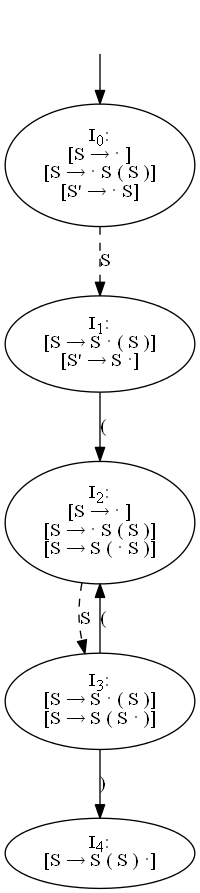
\includegraphics[scale=0.35]{examples/exampleLR0M.png}
	\centering
    \caption{LR(0) statemachine for examples/example.gra}
    \label{lrmex}
\end{figure}

\begin{table}[H]
    \begin{tabular}{| c | c | c | c || c |}
  \hline
  State & ( & ) & \$  & S \\ \hline
  I$_{0}$ & \shortstack{reduce S $\rightarrow$  $\epsilon$} & \shortstack{reduce S $\rightarrow$  $\epsilon$} & \shortstack{reduce S $\rightarrow$  $\epsilon$} & \shortstack{I$_{1}$} \\ \hline
  I$_{1}$ & \shortstack{shift I$_{2}$} & \shortstack{} & \shortstack{reduce S' $\rightarrow$  S} & \shortstack{} \\ \hline
  I$_{2}$ & \shortstack{reduce S $\rightarrow$  $\epsilon$} & \shortstack{reduce S $\rightarrow$  $\epsilon$} & \shortstack{reduce S $\rightarrow$  $\epsilon$} & \shortstack{I$_{3}$} \\ \hline
  I$_{3}$ & \shortstack{shift I$_{2}$} & \shortstack{shift I$_{4}$} & \shortstack{} & \shortstack{} \\ \hline
  I$_{4}$ & \shortstack{reduce S $\rightarrow$  S ( S )} & \shortstack{reduce S $\rightarrow$  S ( S )} & \shortstack{reduce S $\rightarrow$  S ( S )} & \shortstack{} \\ \hline
\end{tabular}

	\centering
    \caption{SLR(1) parsing table for examples/example.gra}
    \label{slrex}
\end{table}

\newpage
Lastly let's generate the LR(1) state machine with TINY states along with a table of the omitted information for each state:
\begin{lstlisting}[frame=single]
java -jar PTG.jar examples/example.gra -LR1M tiny tikz
\end{lstlisting}


\begin{figure}[H]
    \centering
	\begin{tabular}{l r}
        \begin{minipage}{2in}
			\begin{tikzpicture}[>=stealth',shorten >=1pt,auto,node distance=2cm,every text node part/.style={align=center}]
  \node[initial,state]  (i0)  {$I_0$};
  \node[state]  (i1)  [below of=i0]  {$I_{1}$};
  \node[state]  (i2)  [below of=i1]  {$I_{2}$};
  \node[state]  (i3)  [below of=i2]  {$I_{3}$};
  \node[state]  (i4)  [below of=i3]  {$I_{4}$};
  \node[state]  (i5)  [right of=i4]  {$I_{5}$};
  \node[state]  (i6)  [below of=i4]  {$I_{6}$};
  \node[state]  (i7)  [below of=i6]  {$I_{7}$};
  \path[->,dashed] (i0) edge [right] node {S} (i1);
  \path[->] (i1) edge [right] node {(} (i2);
  \path[->,dashed] (i2) edge [right] node {S} (i3);
  \path[->] (i3) edge [right] node {(} (i4);
  \path[->] (i3) edge [right] node {)} (i5);
  \path[->,dashed] (i4) edge [right] node {S} (i6);
  \path[->] (i6) edge [bend left] node {(} (i4);
  \path[->] (i6) edge [right] node {)} (i7);
\end{tikzpicture}

		\end{minipage}
		\begin{minipage}{2in}
			\begin{tabular}{| c | c |}
  \hline
  State & Current Rule Set \\ \hline
  I$_{0}$ & \shortstack{S $\rightarrow$  $\cdot$ $\epsilon$, \$  \\ S $\rightarrow$  $\cdot$ $\epsilon$, ( \\ S $\rightarrow$  $\cdot$ S ( S ), \$  \\ S $\rightarrow$  $\cdot$ S ( S ), ( \\ S' $\rightarrow$  $\cdot$ S, \$ } \\ \hline
  I$_{1}$ & \shortstack{S $\rightarrow$  S $\cdot$ ( S ), \$  \\ S $\rightarrow$  S $\cdot$ ( S ), ( \\ S' $\rightarrow$  S $\cdot$ , \$ } \\ \hline
  I$_{2}$ & \shortstack{S $\rightarrow$  $\cdot$ $\epsilon$, ( \\ S $\rightarrow$  $\cdot$ $\epsilon$, ) \\ S $\rightarrow$  $\cdot$ S ( S ), ( \\ S $\rightarrow$  $\cdot$ S ( S ), ) \\ S $\rightarrow$  S ( $\cdot$ S ), \$  \\ S $\rightarrow$  S ( $\cdot$ S ), (} \\ \hline
  I$_{3}$ & \shortstack{S $\rightarrow$  S $\cdot$ ( S ), ( \\ S $\rightarrow$  S $\cdot$ ( S ), ) \\ S $\rightarrow$  S ( S $\cdot$ ), \$  \\ S $\rightarrow$  S ( S $\cdot$ ), (} \\ \hline
  I$_{4}$ & \shortstack{S $\rightarrow$  $\cdot$ $\epsilon$, ( \\ S $\rightarrow$  $\cdot$ $\epsilon$, ) \\ S $\rightarrow$  $\cdot$ S ( S ), ( \\ S $\rightarrow$  $\cdot$ S ( S ), ) \\ S $\rightarrow$  S ( $\cdot$ S ), ( \\ S $\rightarrow$  S ( $\cdot$ S ), )} \\ \hline
  I$_{5}$ & \shortstack{S $\rightarrow$  S ( S ) $\cdot$ , \$  \\ S $\rightarrow$  S ( S ) $\cdot$ , (} \\ \hline
  I$_{6}$ & \shortstack{S $\rightarrow$  S $\cdot$ ( S ), ( \\ S $\rightarrow$  S $\cdot$ ( S ), ) \\ S $\rightarrow$  S ( S $\cdot$ ), ( \\ S $\rightarrow$  S ( S $\cdot$ ), )} \\ \hline
  I$_{7}$ & \shortstack{S $\rightarrow$  S ( S ) $\cdot$ , ( \\ S $\rightarrow$  S ( S ) $\cdot$ , )} \\ \hline
\end{tabular}

		\end{minipage}
    \end{tabular}
    \caption{LR(0) statemachine for examples/example.gra with TINY states along with labels table.}
    \label{lrex}
\end{figure}


In parting, I wish to point out that the full \LaTeX{} source file for this user manual can be found in \verb|doc/UserManual.tex| in the \href{https://github.com/EgillEinarss/PTG}{PTG repository}.

\end{document}
